%%%%%%%%%%%%%%%%%%%%%%%%%%%%%%%%%%%%%%%%%
% Dreuw & Deselaer's Poster
% LaTeX Template
% Version 1.0 (11/04/13)
%
% Created by:
% Philippe Dreuw and Thomas Deselaers
% http://www-i6.informatik.rwth-aachen.de/~dreuw/latexbeamerposter.php
%
% This template has been downloaded from:
% http://www.LaTeXTemplates.com
%
% License:
% CC BY-NC-SA 3.0 (http://creativecommons.org/licenses/by-nc-sa/3.0/)
%
%%%%%%%%%%%%%%%%%%%%%%%%%%%%%%%%%%%%%%%%%

%----------------------------------------------------------------------------------------
%	PACKAGES AND OTHER DOCUMENT CONFIGURATIONS
%----------------------------------------------------------------------------------------

\documentclass[final,hyperref={pdfpagelabels=false}]{beamer}

\usepackage[orientation=portrait,size=a1,scale=1.4]{beamerposter} % Use the beamerposter package for laying out the poster with a portrait orientation and an a1 paper size

\usetheme{I6pd2} % Use the I6pd2 theme supplied with this template

\usepackage[english]{babel} % English language/hyphenation

\usepackage{amsmath,amsthm,amssymb,latexsym} % For including math equations, theorems, symbols, etc

%\usepackage{times}\usefonttheme{professionalfonts}  % Uncomment to use Times as the main font
%\usefonttheme[onlymath]{serif} % Uncomment to use a Serif font within math environments

\boldmath % Use bold for everything within the math environment

\usepackage{booktabs} % Top and bottom rules for tables

\graphicspath{{figures/}} % Location of the graphics files

\usecaptiontemplate{\small\structure{\insertcaptionname~\insertcaptionnumber: }\insertcaption} % A fix for figure numbering

%----------------------------------------------------------------------------------------
%	TITLE SECTION 
%----------------------------------------------------------------------------------------

\title{\Huge Search for a New Heavy Charged Gauge Boson with ATLAS} % Poster title

\author{Ellis Kay} % Author(s)

\institute{Supervisors: Uta Klein \& Carl Gwilliam} % Institution(s)

%----------------------------------------------------------------------------------------
%	FOOTER TEXT
%----------------------------------------------------------------------------------------

\newcommand{\leftfoot}{} % Left footer text

\newcommand{\rightfoot}{ellis.kay@cern.ch} % Right footer text

%----------------------------------------------------------------------------------------

\begin{document}

\addtobeamertemplate{block end}{}{\vspace*{2ex}} % White space under blocks

\begin{frame}[t] % The whole poster is enclosed in one beamer frame

\vspace*{-1ex}

%%%%%%%%%%%%%%%%%%%%%%%%%%%%%%%%%%%%%%%%%%%%%%%%%%%%%%%%
%%%%%%%%%%%%%%%%%%%%%%%%%%%%%%%%%%%%%%%%%%%%%%%%%%%%%%%%
%%%%%%%%%%%%%%%%%%%%%%%%%%%%%%%%%%%%%%%%%%%%%%%%%%%%%%%%
%%%%%%%%%%%%%%%%%%%%%%%%%%%%%%%%%%%%%%%%%%%%%%%%%%%%%%%%


%%%%%%%%%%%%%%%%%%%%%%%%%%%%%%%%%%%%%%%%%%%%%%%%%%%%%%%%
%%%% SET OF TWO COLUMNS 
%%%%%%%%%%%%%%%%%%%%%%%%%%%%%%%%%%%%%%%%%%%%%%%%%%%%%%%%
\cleft{.02}
\cright{.47}
%%%%%%%%%%%%%%%%%%%%%%%%%%
%----------------------------------------------------------------------------------------
%	INTRODUCTION
%----------------------------------------------------------------------------------------
            
\begin{block}{1 Introduction}

\cleft{.6}
\li{The \wprime is a new gauge boson arising from extensions of electroweak symmetry.	}

\vspace{10pt}
\li{Predicted in a wealth of BSM theories:}
	\lii{Little Higgs {\scriptsize \color{ATLASBlue} (hierarchy problem)}}
	\lii{Left-Right Symmetric {\scriptsize \color{ATLASBlue} (GUT)}}
	\lii{331 Models {\scriptsize \color{ATLASBlue} (3 quark families)}}
	

	
\cright{.38}
    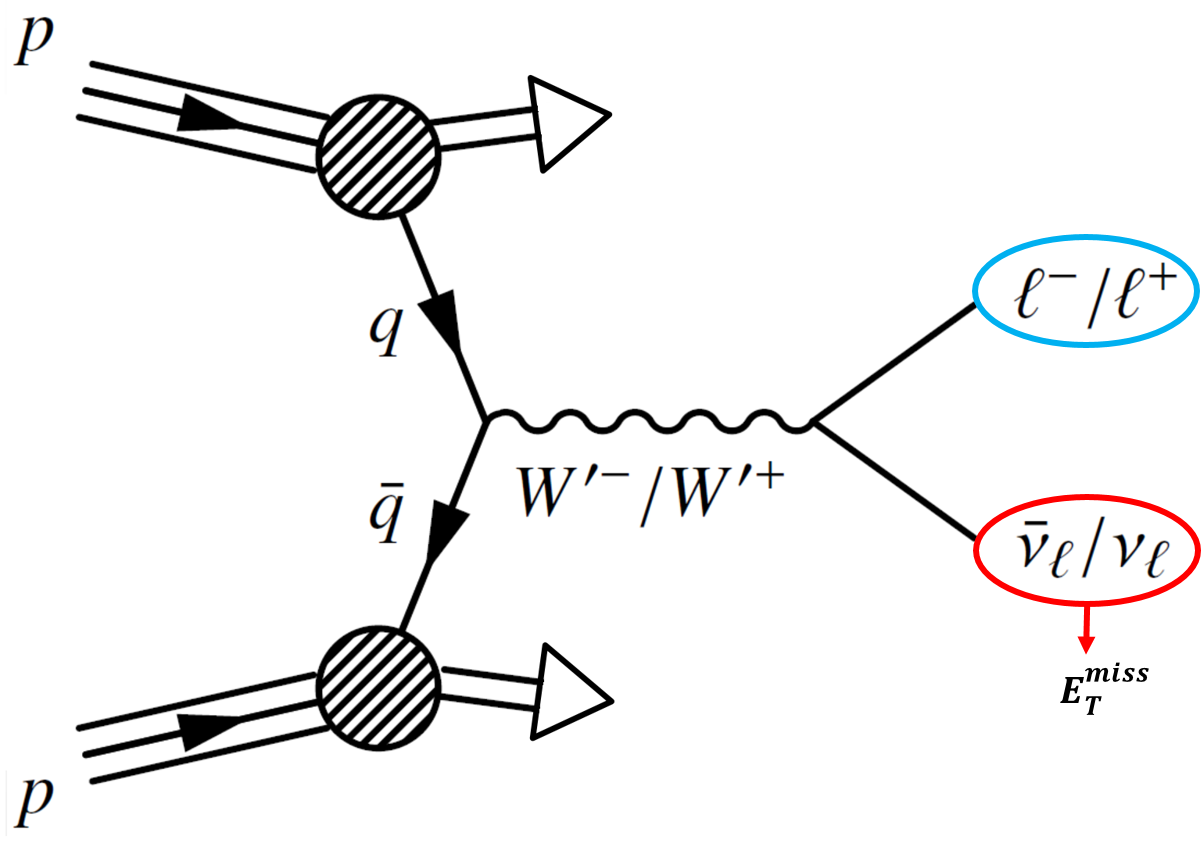
\includegraphics[width=.99\linewidth]{Wprime_feynman_colsMET.png}

\cend 

\vspace{10pt}
\li{We consider spin-1 s-channel \wprime resonances in the context of the Sequential Standard Model (SSM) \cite{SSM}.}
		\lii{Same couplings to fermions as the SM W, TeV scale mass.}
		%\lii{Neglect interference with SM W.}
		%\lii{Very general benchmark model, others may be studied.}
\li{Identify events with one high-\pt\, {\color{ATLASBlue}lepton} and large {\color{red}\met}}
	
	\li{Search for deviations from SM in $\mt = \sqrt{2 {\color{ATLASBlue}\pt} {\color{red}\met} \big( 1 - \cos{\color{purple}\phi_{\ell\nu}} \big) }$}
	\li{For the electron channel \,$\rightarrow$\, $e$: \pt\,>\,65 GeV, \met\,>\,65 GeV, \mt\,>\,130 GeV}

\vspace{.75ex}
\end{block}

%%%%%%%%%%%%%%%%%%%%%%%%%%
\cright{.02}
\cright{.47}
%%%%%%%%%%%%%%%%%%%%%%%%%%
%----------------------------------------------------------------------------------------
%	SAMPLES
%----------------------------------------------------------------------------------------

\begin{block}{2 Samples}
\cleft{.5}
\li{Using the full 36.1 fb\textsuperscript{-1} of 2015+2016 ATLAS data.}
\vspace{10pt}
\li{``Flat" \wprime signal samples (PYTHIA) are reweighted to the desired pole mass.}
%\lii{Generated with the Breit-Wigner term removed}

\vspace{10pt}
\li{SM backgrounds estimated with Monte Carlo include:}	
\cright{.45}
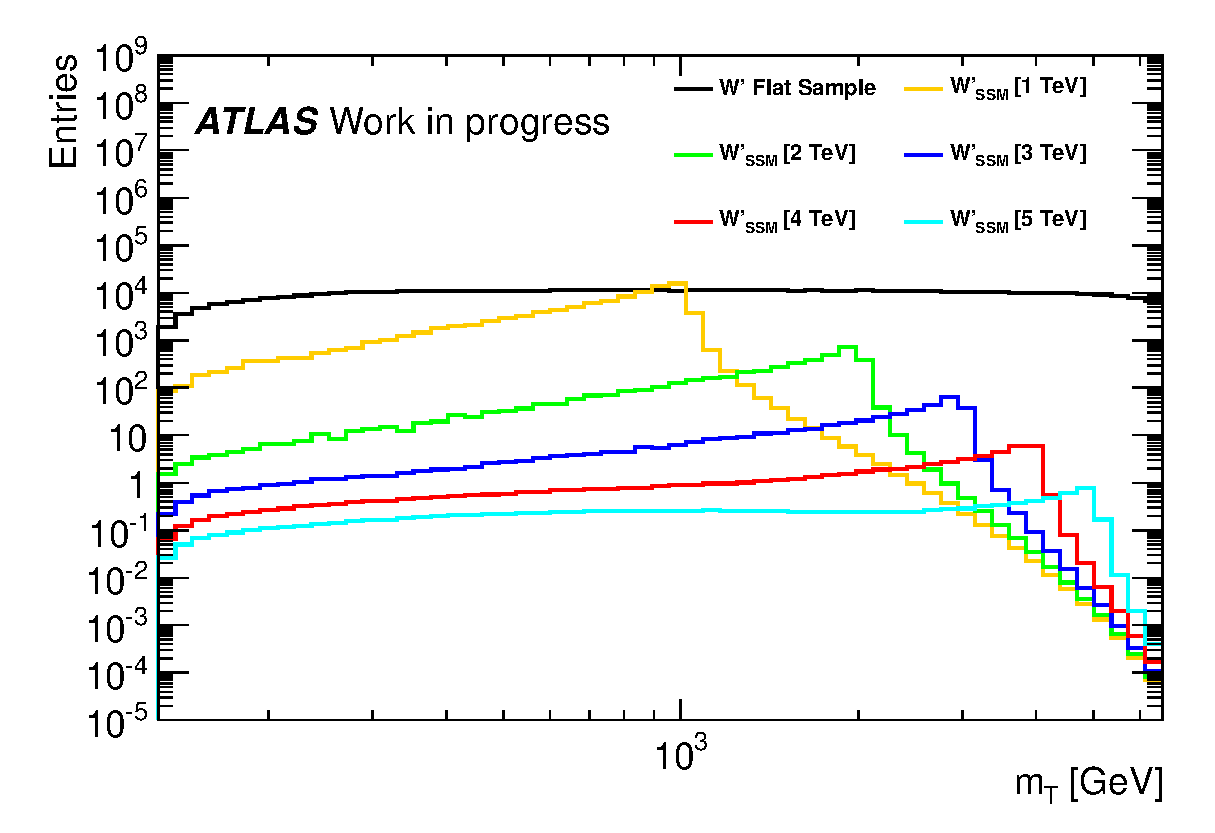
\includegraphics[width=\linewidth]{SignalTemplates.eps}

\cend


	
	\lii{Charged Current Drell-Yan (CCDY) $W \rightarrow e \nu$\ $\star$ {\color{ATLASBlue}(mass-binned)} }
	\lii{Neutral Current Drell-Yan (NCDY) $Z \rightarrow \ell \ell$ $\star$ {\color{ATLASBlue}(mass-binned)}}
	\lii{Top ($t\bar{t}$ \& single top) $\star$ {\color{ATLASBlue}(inclusive)}}
	\lii{Diboson $\dagger$ {\color{ATLASBlue}(inclusive)}}
{\footnotesize $\star$ - Powheg \& Pythia8, $\dagger$ - Sherpa.}
\vspace{5pt}
\li{`Multijet' background is estimated using data-driven methods.}

\vspace{.7ex}
\end{block}

%%%%%%%%%%%%%%%%%%%%%%%%%%
\cright{.02}
\cend
%\vspace*{2ex}

%%%%%%%%%%%%%%%%%%%%%%%%%%%%%%%%%%%%%%%%%%%%%%%%%%%%%%%%
%%%% SINGLE COLUMN
%%%%%%%%%%%%%%%%%%%%%%%%%%%%%%%%%%%%%%%%%%%%%%%%%%%%%%%%
\cleft{.02}
\cright{.96}
%%%%%%%%%%%%%%%%%%%%%%%%%%
%----------------------------------------------------------------------------------------
%	FAKE LEPTON BACKGROUND
%----------------------------------------------------------------------------------------

\begin{block}{3 ``Fake" Lepton Background}

\cleft{.45}
\li{SM Background due to misidentified leptons in multijet processes ("fake" leptons) are poorly described by MC}
	%\lii{$\rightarrow$ use a data-driven Matrix Method.}
	\li{Use a data-driven Matrix Method:}
		\lii{Exploits the different
probabilities for ``real'' and ``fake'' leptons to
pass from ``loose'' to ``tight'' cuts}
		\lii{Using {\color{orange}measurable} quantities to calculate {\color{purple}truth} quantities}
			
		\vspace{5pt}
		%\begin{center}\makebox[.7\textwidth][c]{%
		\begin{minipage}{.5\linewidth}
			\begin{equation*}
			\psBox{orange!30}{
  		  		\begin{pmatrix} 
				N_{T} \\
				N_{L} 
				\end{pmatrix}
				}=
				\begin{pmatrix}
				\epsilon_{R} & \epsilon_{F} \\
				1 - \epsilon_{R} & 1 - \epsilon_{F}
				\end{pmatrix}
				\psBox{purple!30}{
				\begin{pmatrix}
				N_{R} \\
				N_{F}
				\end{pmatrix}
				}
 		 	\end{equation*} 
		\end{minipage}\hfill
		\begin{minipage}{.4\linewidth}
			\begin{equation*}
			\boxed{
 				\epsilon_{F} = \frac{N^{fake}_{tight}}{N^{fake}_{loose}}, \, \,  
 				\epsilon_{R} = \frac{N^{real}_{tight}}{N^{real}_{loose}}
 				}
  			\end{equation*}
		\end{minipage}
		%} \end{center}		
		
\vspace{-5pt}
	{\footnotesize \phantom{x}\hspace{27ex} {\color{ATLASBlue}signal selection} \hspace{5ex} {\color{red}contribution from fake electrons} }
	\vspace{-9pt}
	\li{From the first line: \hspace{5ex}$\highlight[ATLASBlue_lighter]{N_{T}} = \highlight[highgreen]{\epsilon_{R}N_{R}} + \highlight[highred]{\epsilon_{F}N_{F}}$ }
	\vspace{-25pt}
	{\footnotesize \phantom{x}\hspace{33ex} {\color{green}contribution from real electrons} }
\vspace{5pt}
	\li{Inverting matrix yields ``fake'' component in data (tight selection):}
\vspace{10pt}
		\begin{equation*}
			\epsilon_{F}N_{F} = \frac{\epsilon_{F}}{\epsilon_{R} - \epsilon_{F}} \big[ \epsilon_{R}(N_{L} + N_{T}) - N_{T} \big]	
		\end{equation*}
		
\cright{.5}

\li{``tight“ selection $\rightarrow$ signal selection}
\li{``loose” selection $\rightarrow$ as loose as possible, containing ``tight” electrons}
\li{``loose” level $\rightarrow$ loosest unprescaled trigger which collects this sample}
\vspace{-20pt}
\cleft{.5}
{\footnotesize \phantom{x}\hspace{10ex} HLT\_e140\_lhloose for \pt $>$ 145 GeV }
\cright{.5}
{\footnotesize \phantom{x}\hspace{8ex} HLT\_e60\_lhmedium for \pt $<$ 145 GeV }
\cend

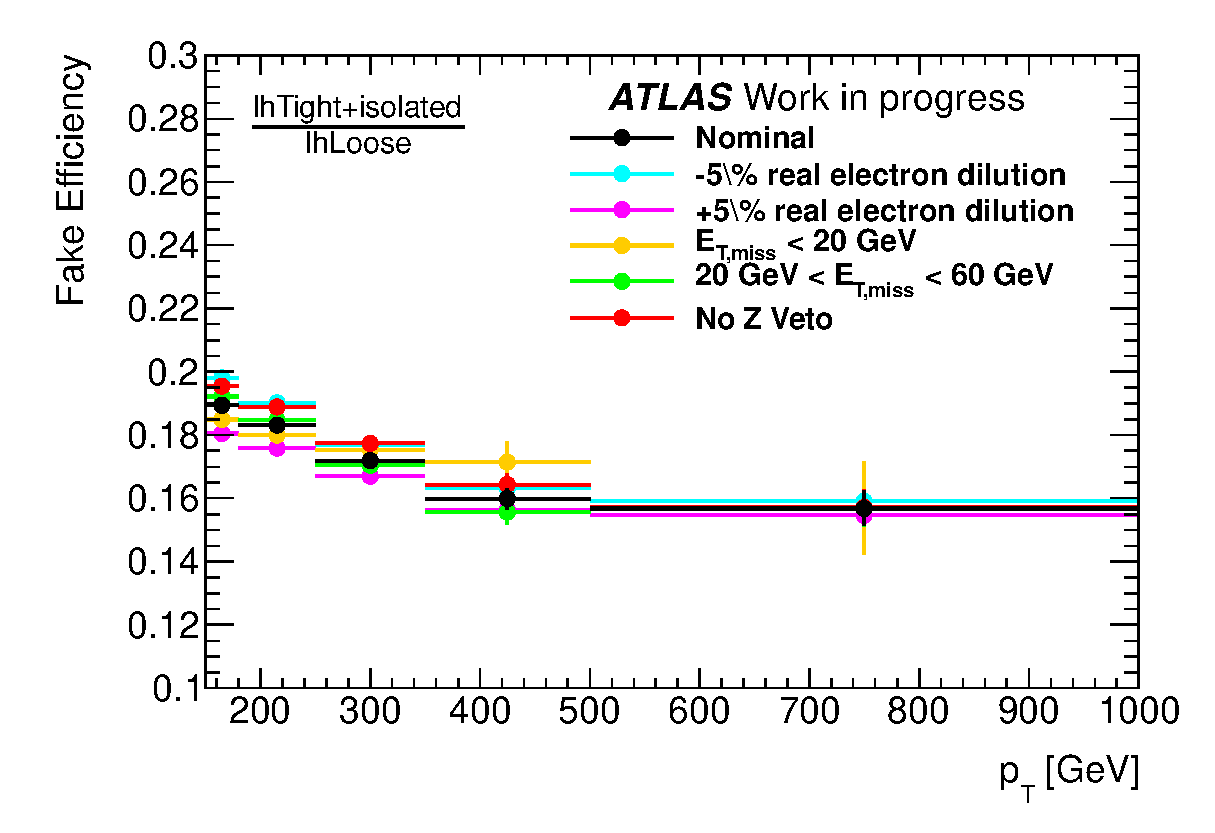
\includegraphics[width=.5\linewidth]{RFplots/TL_FakeRate_pt_F.eps}
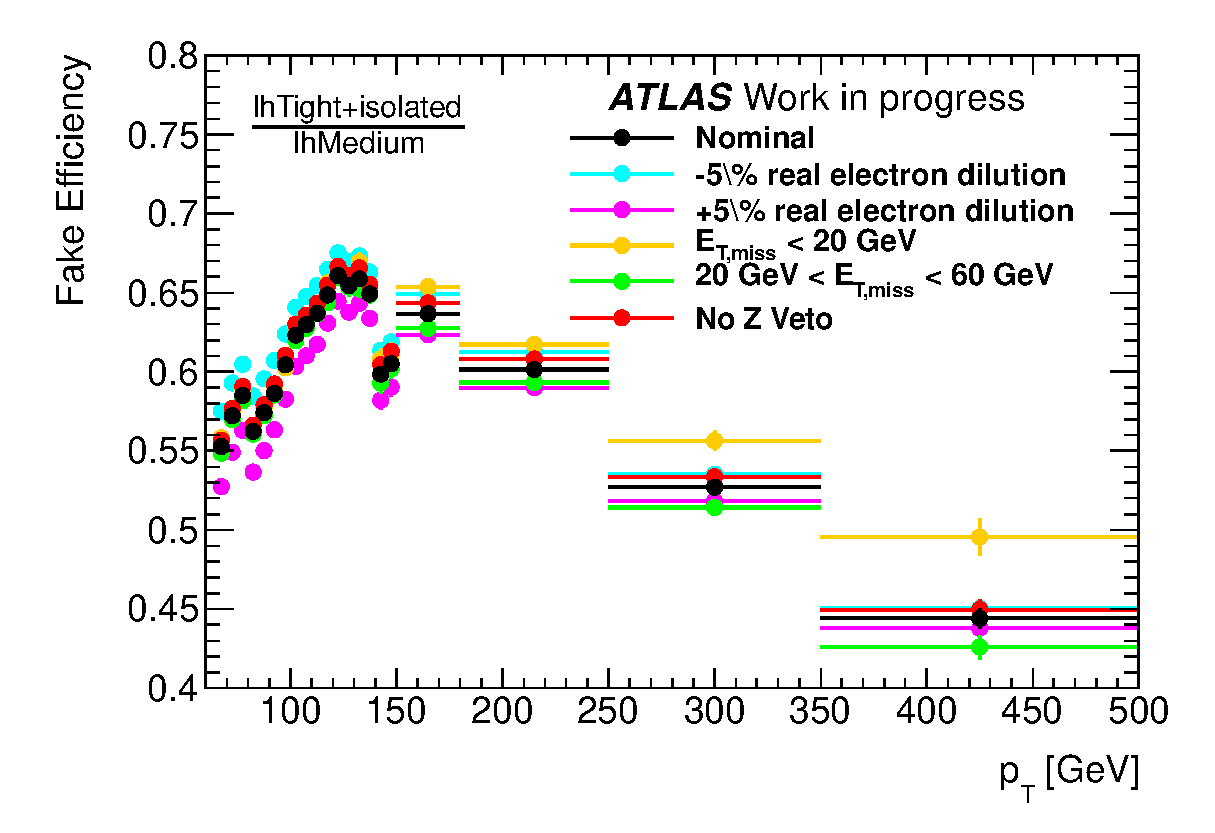
\includegraphics[width=.5\linewidth]{RFplots/TM_FakeRate_pt_F.eps}
\vspace{-35pt}
\li{The selections which define the multijet control region for $\epsilon_{F}$\, are varied to obtain a systematic uncertainty on this background.}
\cend

\vspace{.75ex}
\end{block}

%%%%%%%%%%%%%%%%%%%%%%%%%%
\cright{.02}
\cend
%\vspace*{2ex}

%%%%%%%%%%%%%%%%%%%%%%%%%%%%%%%%%%%%%%%%%%%%%%%%%%%%%%%%
%%%% SET OF TWO COLUMNS
%%%%%%%%%%%%%%%%%%%%%%%%%%%%%%%%%%%%%%%%%%%%%%%%%%%%%%%%
\cleft{.02}
\cright{.4}
%%%%%%%%%%%%%%%%%%%%%%%%%%
%----------------------------------------------------------------------------------------
%	HIGHER-ORDER CORRECTIONS
%----------------------------------------------------------------------------------------

\begin{block}{4 Theoretical Uncertainties}


\li{Signal \& dominant CCDY background samples are corrected to best theory knowledge:}

\cleft{.45}
\lii{Signal $\rightarrow$\, NNLO\textsubscript{QCD}}
\cright{.55}
\lii{CCDY $\rightarrow$\, NNLO\textsubscript{QCD} \& NLO\textsubscript{EW}}
\cend

\vspace{20pt}
\li{For searches at the TeV scale, understanding of the parton structure of the proton becomes a dominant source of uncertainty.}

\vspace{20pt}
\li{Additional theoretical uncertainties for background:}
\cleft{.5}
\lii{PDF \& $\alpha_{S}$\, for nominal set}
\cright{.5}
\lii{PDF choice uncertainty}
\cend

\begin{center}
%\begin{figure}
%  \caption{Ratios of the central values and uncertainties for all %modern PDF sets to the CT14 (nominal) central values.}
%  \centering
    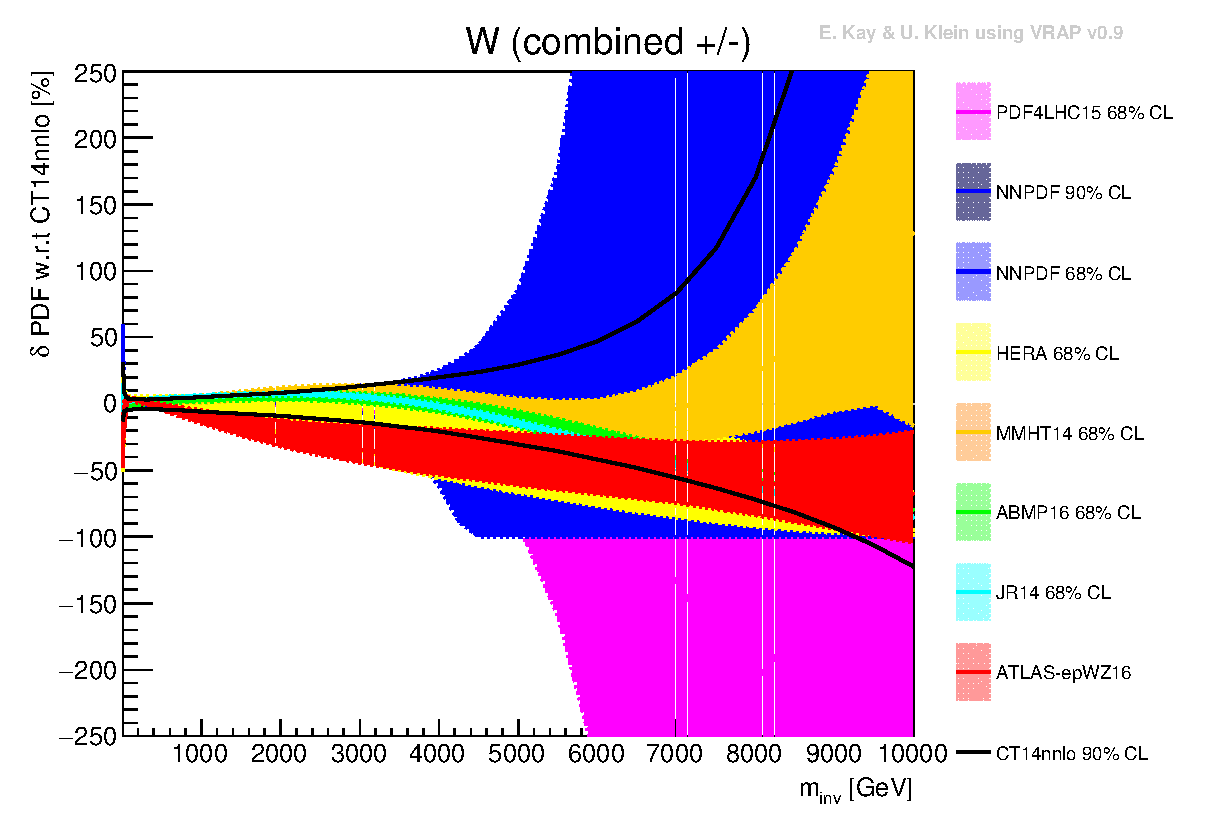
\includegraphics[width=.8\linewidth]{Wcomb.eps}
%\end{figure}
\\{\footnotesize \color{ATLASBlue} {Ratios of the central values and uncertainties at NNLO QCD for all modern PDF sets to the CT14 (nominal) central values for the CCDY process.}}

\end{center}
\vspace{-5pt}
\vspace{.75ex}
\end{block}



%%%%%%%%%%%%%%%%%%%%%%%%%%
\cright{.02}
\cright{.54}
%%%%%%%%%%%%%%%%%%%%%%%%%%
%----------------------------------------------------------------------------------------
%	RESULTS & CONCLUSIONS
%----------------------------------------------------------------------------------------

\begin{block}{5 Results}
\cleft{.52}
\begin{center}
	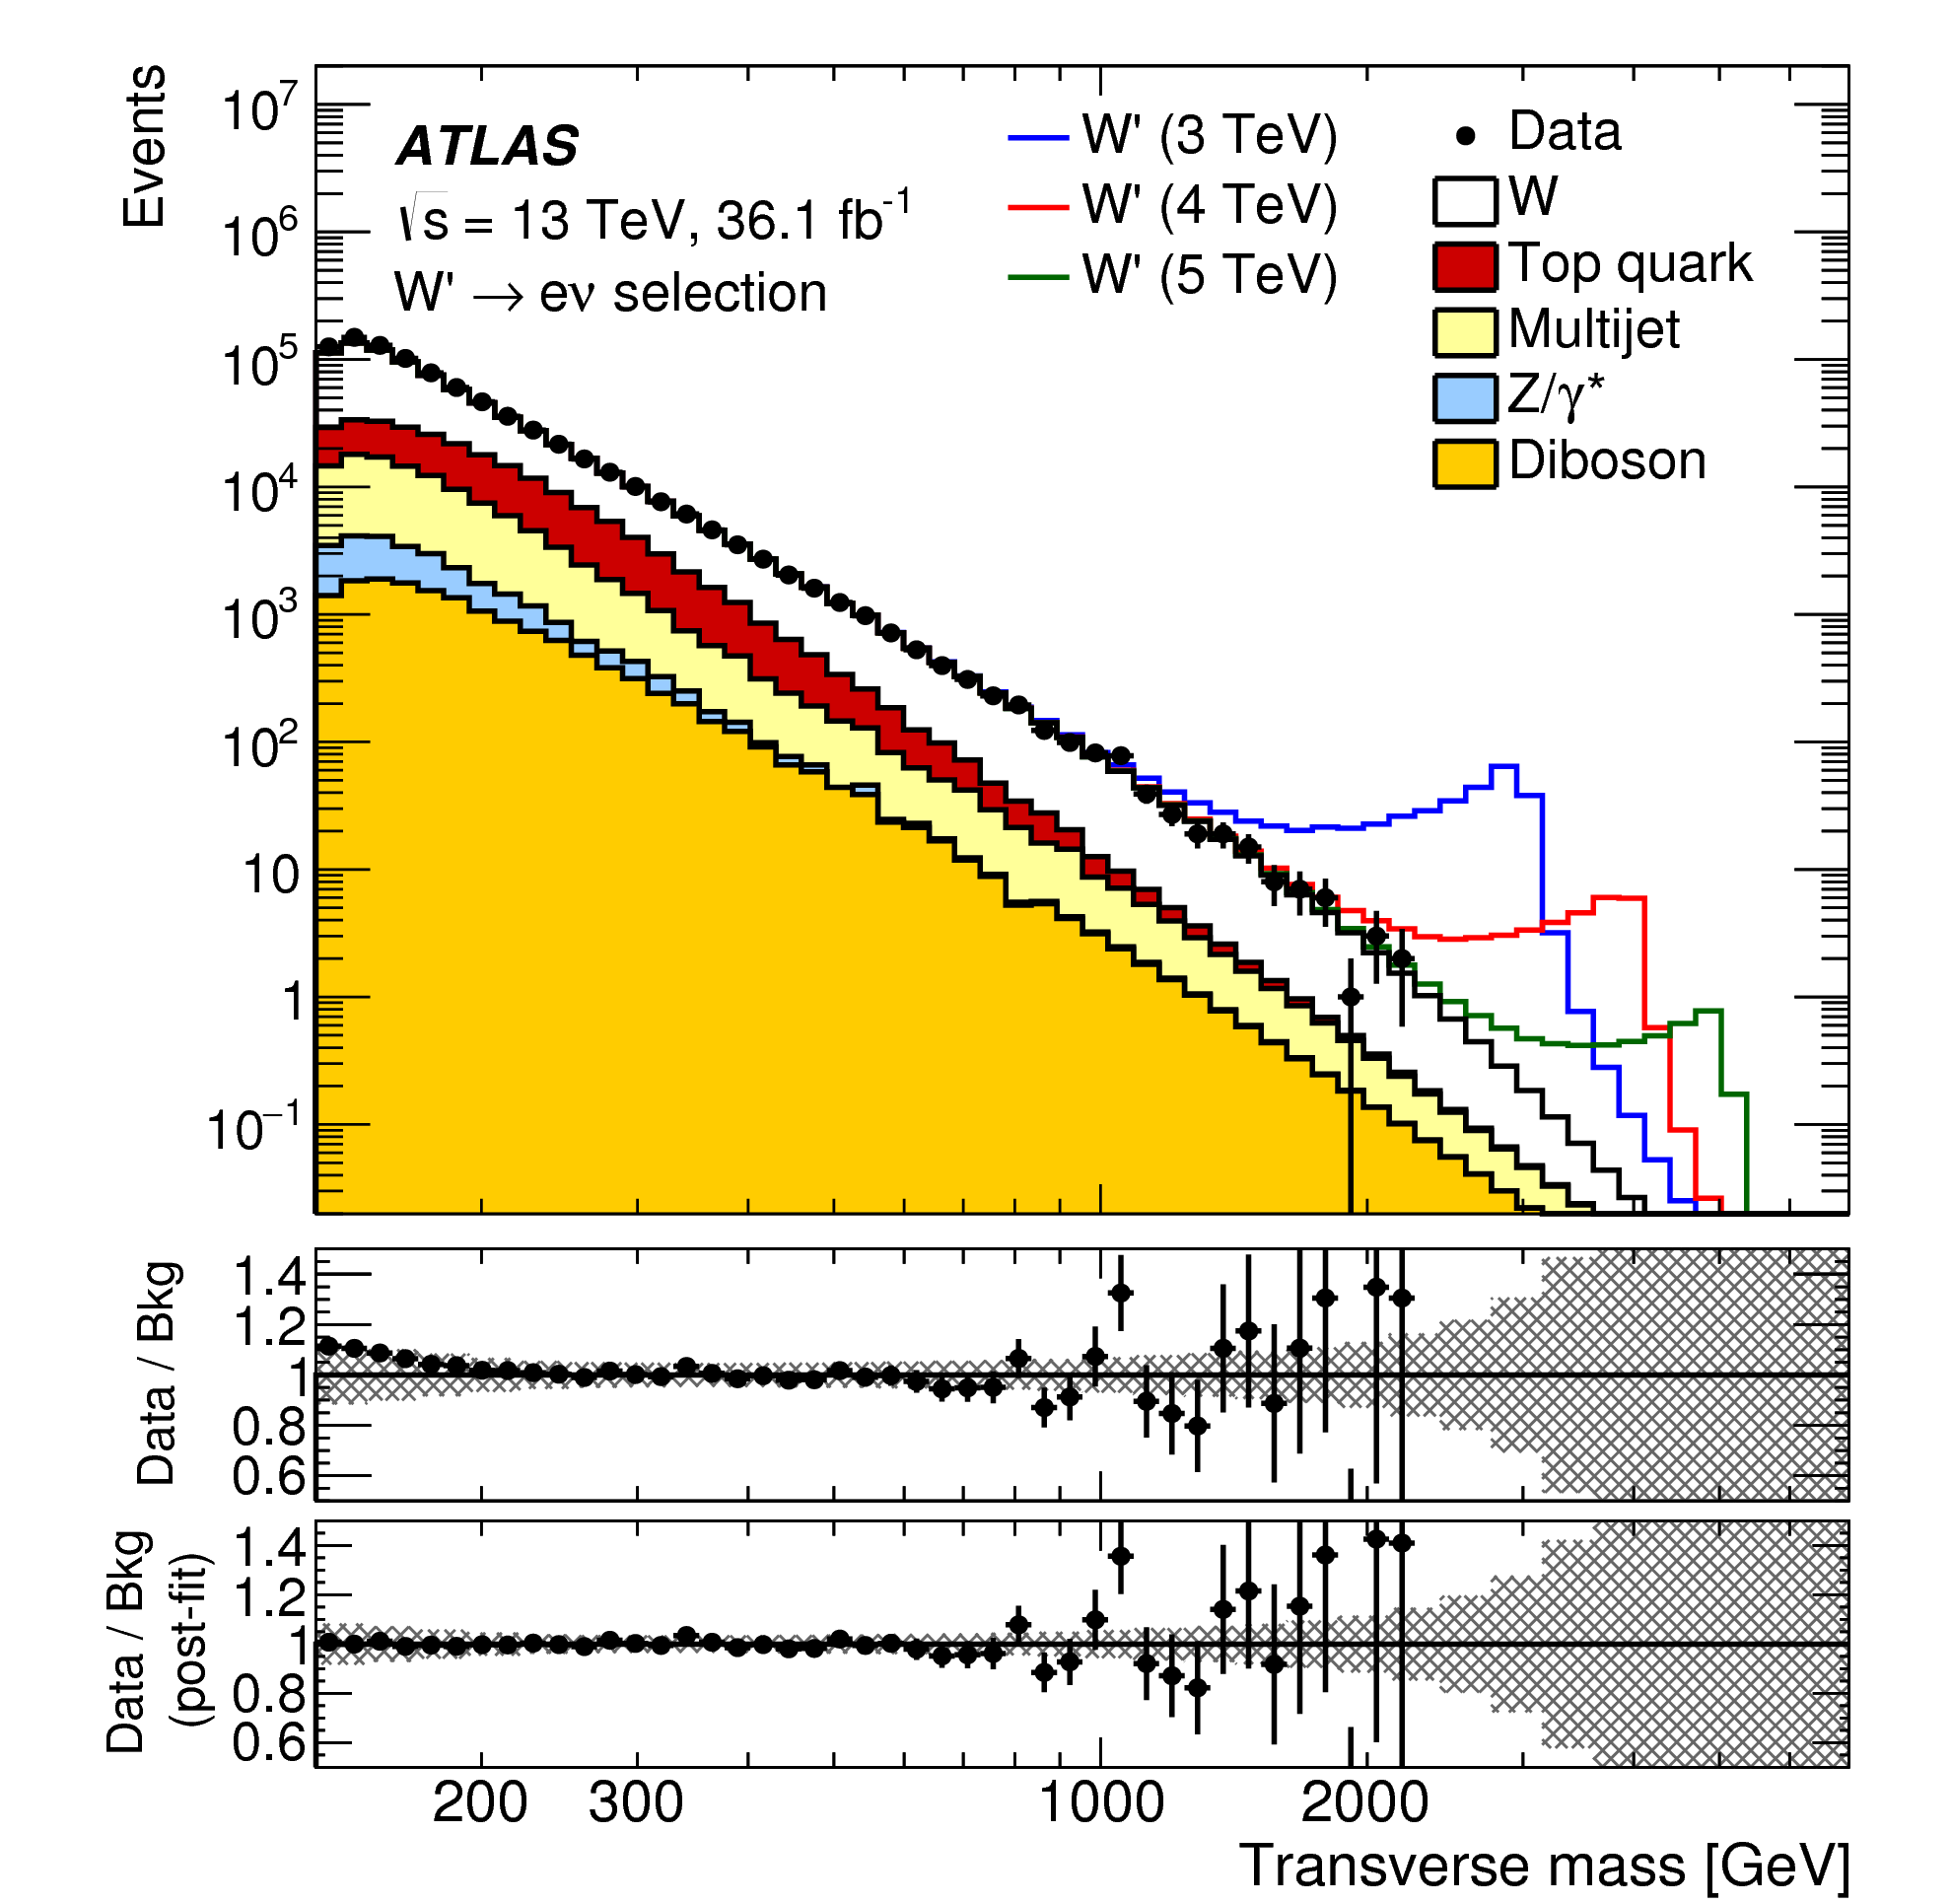
\includegraphics[width=\linewidth]{mT_enu_arXiv.png}
\end{center}
\cright{.45}
\vspace{50pt}
%\begin{center}
	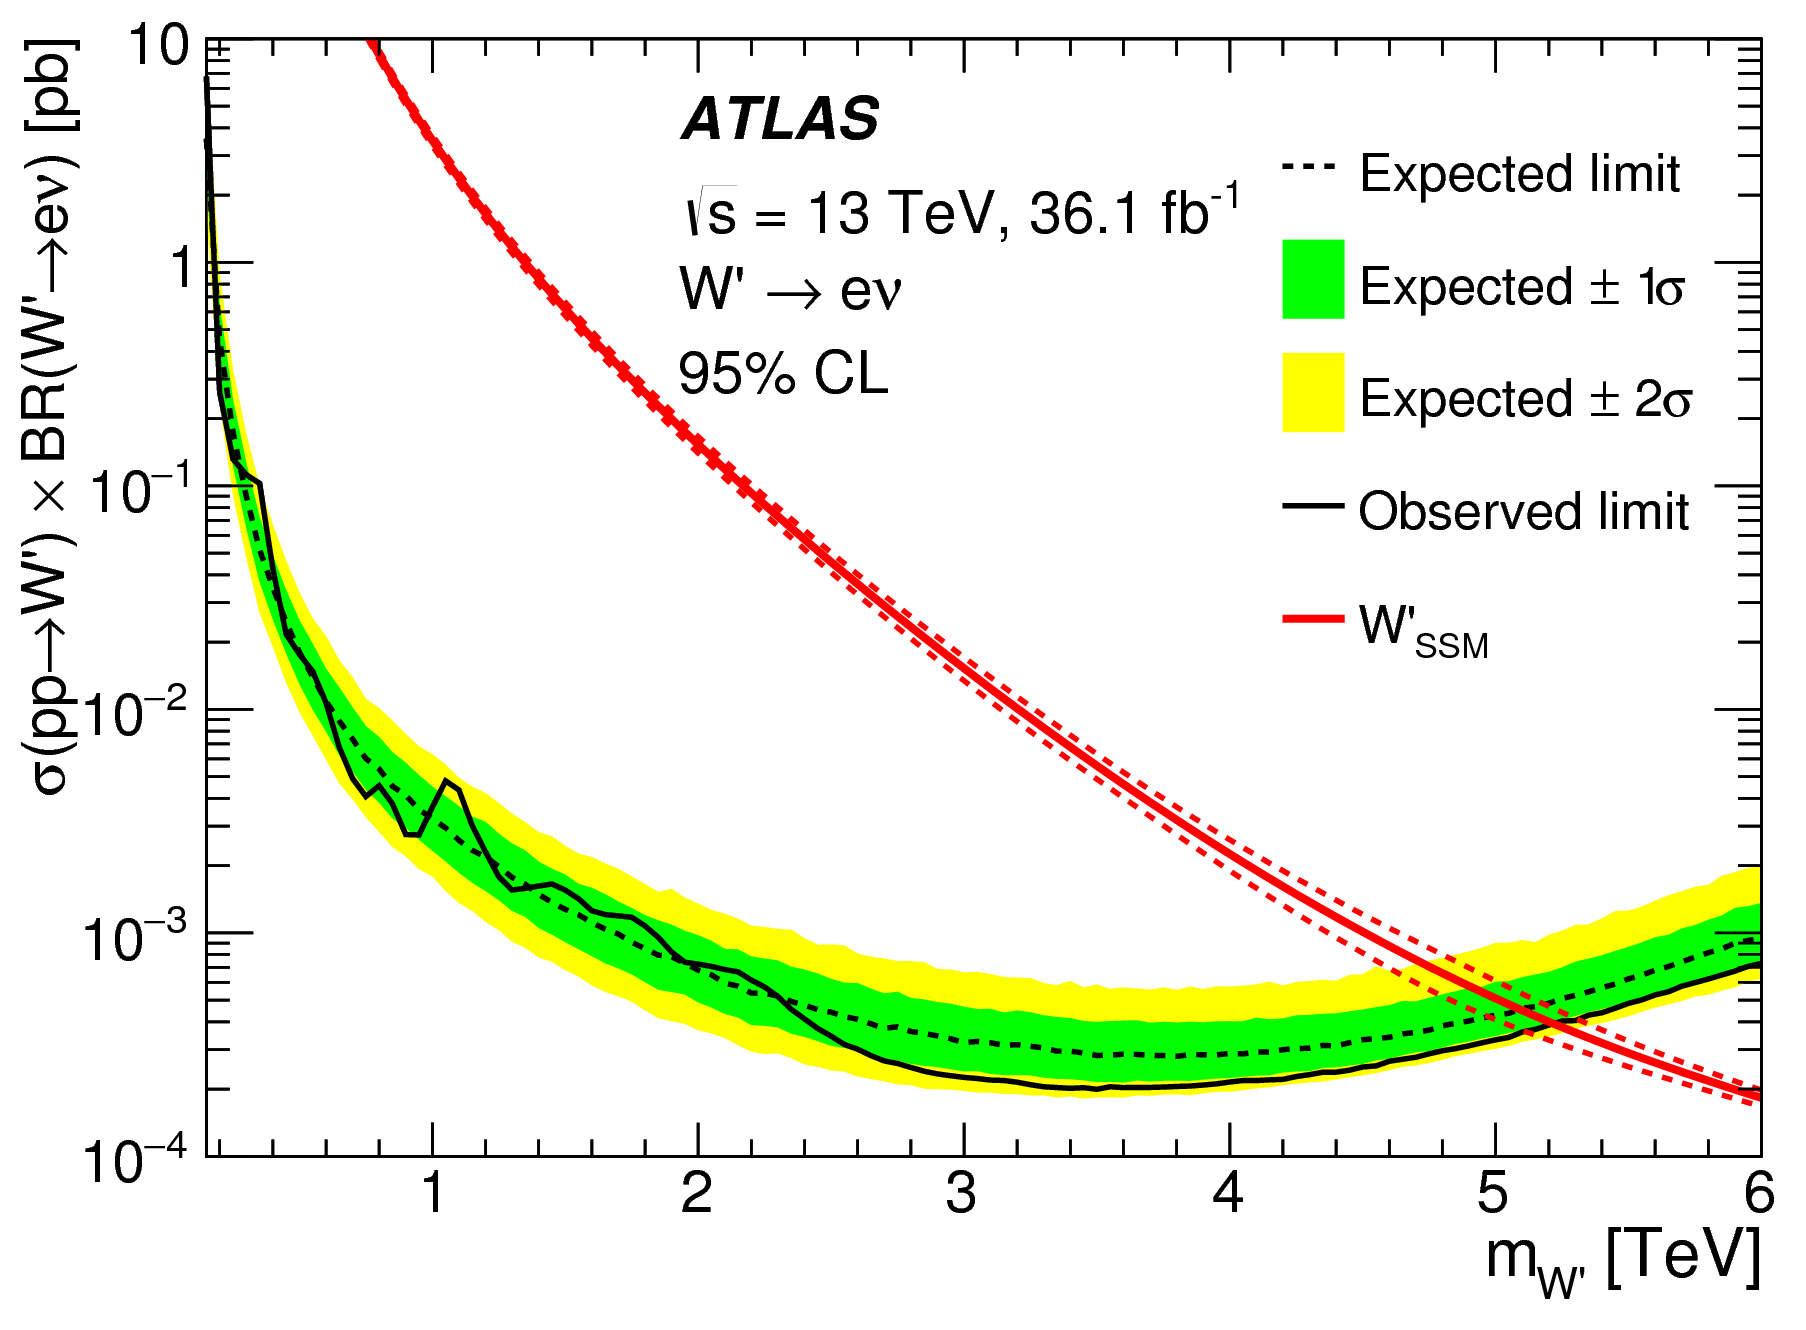
\includegraphics[width=\linewidth]{limit_enu_arXiv.png}
%\end{center}
\li{No significant excess above the SM is observed.}
\li{Limits are set using the Bayesian Analysis Toolkit \cite{BAT}.}

\cright{.01}
\cend


\vspace{20pt}
\li{\wprime SSM masses below 5.2 TeV are excluded at 95\% confidence level for the electron channel.}
\li{This result was published on arXiv \cite{paper}.}
\vspace{20pt}
\li{This search could be strengthened through combination with other analyses, such as \zprime\,searches and searches with \wprime decays to dibosons.}
\lii{Work is in progress to also set frequentist limits in order to facilitate such combinations.}

\vspace{.75ex}
\end{block}


%%%%%%%%%%%%%%%%%%%%%%%%%%
\cright{.02}
\cend
%\vspace*{2ex}

\vspace{-25pt}

%%%%%%%%%%%%%%%%%%%%%%%%%%%%%%%%%%%%%%%%%%%%%%%%%%%%%%%%%
%%%%% SINGLE COLUMN
%%%%%%%%%%%%%%%%%%%%%%%%%%%%%%%%%%%%%%%%%%%%%%%%%%%%%%%%%
%\cleft{.02}
%\cright{.96}
%%%%%%%%%%%%%%%%%%%%%%%%%%%
%\begin{block}{References}
{\footnotesize
	\bibliographystyle{ieeetr}
	\bibliography{posterBIB}
}
%\end{block}
%%%%%%%%%%%%%%%%%%%%%%%%%%%
%\cright{.02}
%\cend
\vspace*{2ex}

%%%%%%%%%%%%%%%%%%%%%%%%%%%%%%%%%%%%%%%%%%%%%%%%%%%%%%%%
%%%%%%%%%%%%%%%%%%%%%%%%%%%%%%%%%%%%%%%%%%%%%%%%%%%%%%%%
%%%%%%%%%%%%%%%%%%%%%%%%%%%%%%%%%%%%%%%%%%%%%%%%%%%%%%%%
%%%%%%%%%%%%%%%%%%%%%%%%%%%%%%%%%%%%%%%%%%%%%%%%%%%%%%%%

\end{frame} % End of the enclosing frame

\end{document}
